\chapter{Synthèse de circuits et Quine Mc.Cluskey}
\section{Synthèse des circuits à partir de spécification verbales}
\paragraph{Spécification formelle} Description complète, précise et non-ambiguë de toutes les propriétés d'un système (TdV, K-Map etc.).
\paragraph{Combinatoire} Les sorties du système ne dépendent que des entrées.\\

Si le problème \textbf{est combinatoire}, alors on peut appliquer tout ce qui a été vu jusqu'à présent.\\
N.B. : commencer par déterminer le nombre d'entrées et de sorties
\section{Additionneurs re-visités}
On souhaite réaliser un circuit additionneur de deux mots A et B codés sur 4 bits (peut généraliser pour $n$ bits).\\
deux solutions s'offrent à nous:
\begin{itemize}
	\item Mimer le principe d'addition bit à bit (séquence de calcul dans le temps)
	\item Anticiper le report pour un certain nombre de bits (considérer le problème comme combinatoire)
\end{itemize}
\subsection{Addition bit à bit}
\label{subsec:addbitàbit}
L'addition est faite grâce à:
\begin{itemize}
	\item un 1/2 additionneur (deux opérantes d'un bit, deux bits d'entrées)
	\item $(n-1)\times$ additionneur complet (deux opérantes d'un bit + un bit de report d'une étage précédent, trois bits d'entrées)
\end{itemize}
\begin{minipage}{.45\textwidth}
	\begin{figure}[H]
		\centering
		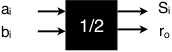
\includegraphics[width=.6\textwidth]{ch5/image1}
	\end{figure}
\end{minipage}
\begin{minipage}{.55\textwidth}
	\begin{figure}[H]
		\centering
		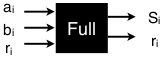
\includegraphics[width=.48\textwidth]{ch5/image2}
	\end{figure}
\end{minipage}
\begin{minipage}[t]{.25\textwidth}
	\begin{table}[H]
		\centering
		$\begin{array}{|c|c|c|c}
			\cline{1-3}
			S_i & 0 & 1 & b_i\\
			\cline{1-3}
			0 & 0 & 1 & \\
			\cline{1-3}
			1 & 1 & 0 & \\
			\cline{1-3}
			\multicolumn{1}{c}{a_i} & \multicolumn{1}{c}{ } & \multicolumn{1}{c}{ }		
		\end{array}$
		\begin{align*}
			S_i &=a_i'b_i+a_ib_i'\\
			&= a_i  \oplus b_i
		\end{align*} 
	\end{table}

\end{minipage}
\begin{minipage}[t]{.2\textwidth}
	\begin{table}[H]
		\centering
		$\begin{array}{|c|c|c|c}
			\cline{1-3}
			r_0 & 0 & 1 & b_i\\
			\cline{1-3}
			0 & 0 & 0 & \\
			\cline{1-3}
			1 & 0 & 1 & \\
			\cline{1-3}
			\multicolumn{1}{c}{a_i} & \multicolumn{1}{c}{ } & \multicolumn{1}{c}{ }		
		\end{array}$
		\begin{equation*}
			r_0 = a_ib_i
		\end{equation*} 
	\end{table}
\end{minipage}
\begin{minipage}[t]{.3\textwidth}
	\begin{table}[H]
		\centering
		$\begin{array}{|c|c|c|c|c|c}
			\cline{1-5}
			S & 00 & 01 & 11 & 10 & a_ib_i\\
			\cline{1-5}
			0 & 0 & 1 & 0 & 1 & \\
			\cline{1-5}
			1 & 1 & 0 & 1 & 0 & \\
			\cline{1-5}
			\multicolumn{1}{c}{r_i} & \multicolumn{1}{c}{ } & \multicolumn{1}{c}{ } & \multicolumn{1}{c}{ } & \multicolumn{1}{c}{ } & \multicolumn{1}{c}{ } 	
		\end{array}$
		\begin{equation*}
			S = a_i\oplus b_i\oplus r_i
			\end{equation*} 
	\end{table}
\end{minipage}
\begin{minipage}[t]{.3\textwidth}
	\begin{table}[H]
		\centering
		$\begin{array}{|c|c|c|c|c|c}
			\cline{1-5}
			r & 00 & 01 & 11 & 10 & a_ib_i\\
			\cline{1-5}
			0 & 0 & 0 & 1 & 0 & \\
			\cline{1-5}
			1 & 0 & 1 & 1 & 1 & \\
			\cline{1-5}
			\multicolumn{1}{c}{r_i} & \multicolumn{1}{c}{ } & \multicolumn{1}{c}{ } & \multicolumn{1}{c}{ } & \multicolumn{1}{c}{ } & \multicolumn{1}{c}{ } 	
		\end{array}$
		\begin{equation*}
			r = a_ib_i+r_ib_i+r_ia_i
		\end{equation*} 
	\end{table}
\end{minipage}
Ainsi, pour un additionneur complet sur 4 bits:
\begin{figure}[H]
	\centering
	
\includegraphics[scale=0.7]{ch5/image3}
\end{figure}
Le problème de ce système est la propagation du report entre les étages: le résultat final sera obtenu après la propagation du report à travers tous les étages de l’additionneur ($n$-délais).
\subsection{Additionneur \textit{Carry Look Ahead} (CLA)}
Le principe est de faire de faire un additionneur complet en un seul circuit combinatoire, permettant d'éviter le problème de délais du à la propagation du report en l'anticipant(\textit{Carry Look Ahead}).\\
Le problème étant combinatoire avec 4 entrées (4 bits) et 3 sorties ($(11)_2+(11)_2=(110)_2$), nous pouvons faire nos K-Maps:\\
\begin{figure}[H]
	\centering
	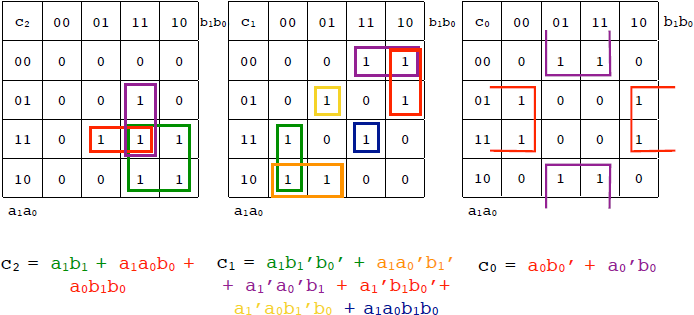
\includegraphics[width=\textwidth]{ch5/image4}
\end{figure}
Pour un plus grand nombre de bits (32, 64 etc.), on préfère mettre en série car si $\nearrow$ entrées/sorties $\rightarrow \nearrow$ taille du circuit (mémoire) $\Rightarrow$ explosion combinatoire.\\
Il y aura un délai de report du à la mise en série, mais moindre que le système vu en \autoref{subsec:addbitàbit}
\section{Encodeurs de priorité}
Un mot D est codé sur $n$ bits. On veut connaître l'index du bit de poids le plus fort ayant un «1» et signaler la présence d'un 1 par un signal ANY.\\

Pour un mot à 4 bits:
\begin{itemize}
	\item 4 entrées
	\item 3 sorties:
	\begin{itemize}
		\item 2 bits pour coder l'index (index max $=4$) 
		\item 1 bit pour le ANY
	\end{itemize}
\end{itemize}
\begin{figure}[H]
	\centering
	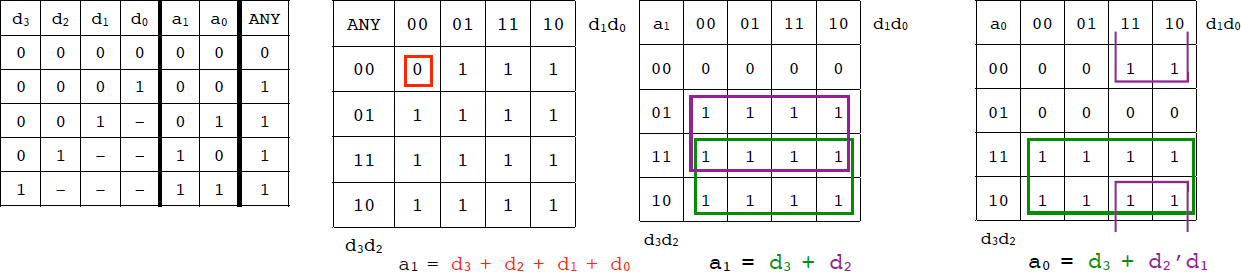
\includegraphics[width=\textwidth]{ch5/image5}
\end{figure}
\section{Simplification des fonctions : Méthode Quine-Mc.Cluskey}
La méthode de Quine-Mc.Cluskey est:
\begin{itemize}
	\item méthode systématique, analysant toutes les possibilités de regroupement. 
	\item utilisée pour un grand nombre de variables
	\item garantit la meilleure solution
	\item facilement programmable
\end{itemize}
Elle se base sur 2 étapes:
\begin{enumerate}
	\item Recherche des implicants premiers  par la \textbf{méthode des tris successifs} (phase d'\textbf{analyse})
	\item Couverture de la fonction  par un choix des implicants premiers (phase de \textbf{synthèse})
\end{enumerate}
\subsection{Étape 1: Analyse}
Elle consiste en 9 étapes (oui, dans le cours c'est 11):
\begin{enumerate}
	\item Pour une fonction $f$ de $n$ variables, on construit $m$ groupements de \textbf{tous les mintermes} de la fonction
	\item Dans chaque groupement des mintermes (noté $G_i$)
	\begin{itemize}
		\item $i$ variables qui valent 1
		\item $(n-i)$ qui valent 0
	\end{itemize}
	\begin{figure}[H]
		\centering
		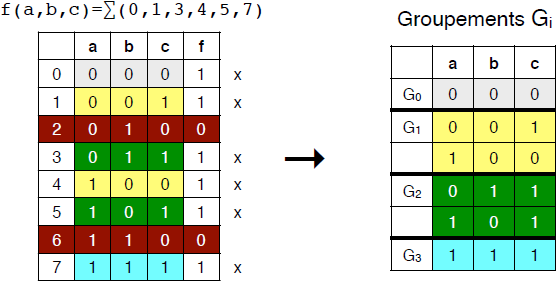
\includegraphics[width=.6\textwidth]{ch5/image6}
	\end{figure}
	\item On compare chaque minterme de $G_i$ avec \textbf{TOUS} les mintermes appartenant à $G_{i+1}$ en termes de la distance de Hamming ($\forall i$)
	\item Si la distance de Hamming entre 2 mintermes $=1$, on les marque par un $x$  et on note \textbf{l'appariement} entre les 2:
	\begin{equation}
		\left.
			\begin{array}{r}
				000\\
				010
			\end{array}
		\right\}\Rightarrow 0\text{-}0
	\end{equation}
	impliquant la possibilité de faire un $n$-cube de plus grande taille (taille 2 à ce stade).\\
	Sinon, il s'agit d'un \textit{impliquant premier} ($n$-cube de taille 1 à ce stade) qu'on notera $IP_k$ dans l'ordre d'apparition
	\item Tous les appariements de $G_i$ et $G_{i+1}$ sont écrits dans un nouveau groupement, noté $G_i'$
	\item Après une première passe, il y a donc au moins $m-1$ groupements $G_i'$
	\item L'ensemble $G_i'$ constitue donc l'ensemble de tous les $n$-cube de taille 2
	\item On répète l'opération avec les nouveaux groupements jusqu'à ce qu'il ne soit plus possible d'apparier
	\item On dresse la liste de tous les implicants premiers (IPs) trouvés.
\end{enumerate}
\subsubsection{Remarques}
\begin{enumerate}
	\item On peut avoir $m=n$
	\item Marquer \textbf{clairement} la séparation entre les $G_i$
	\item Les \textit{don't care} sont également pris en compte pour la distance de Hamming
	\begin{table}[H]
		\centering
		\begin{tabular}{|ccc|}
			\hline
			-000 & Distance de Hamming de 1 & -000\\
			-100 & on \textbf{peut} apparier & -{}-00\\
			\hline
			-000 & Distance de Hamming de 2 & \\
			01-0 & on \textbf{ne peut pas} apparier & \\
			\hline
		\end{tabular}
	\end{table}
	\item S'il y a présence d'indifférent (\textit{don't care}, \textit{don't happen}) au début du problème:
	\begin{itemize}
		\item on fait l'hypothèse qu'ils valent 1 (et donc les rajoutes dans les groupement $G_i$ sans aucune distinction)
		\item Les implicants premiers non-utile (composés que d'indifférents) seront éliminés lors de la 2\up{ème} phase (couverture)
	\end{itemize}
\end{enumerate}
\subsubsection{Exemple}
\begin{figure}[H]
	\centering
	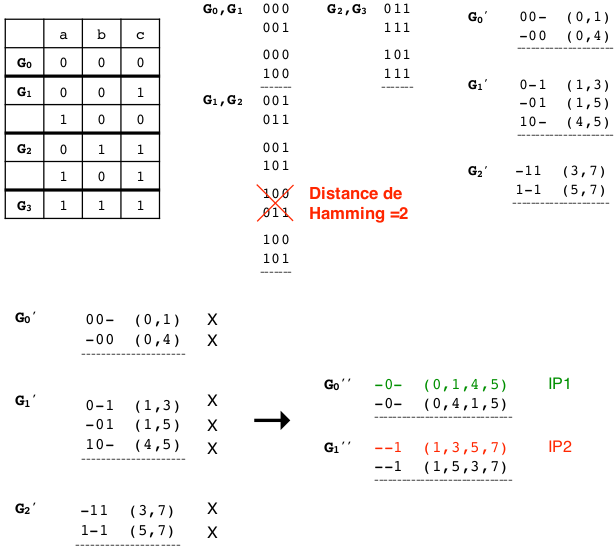
\includegraphics[width=\textwidth]{ch5/image7}
\end{figure}